The Transverse Field Ising (TFI) model is a well-studied spin lattice model that is described by the Hamiltonian
\begin{equation}
	\label{eq:TFI_Hamiltonian}
	\hat{H}_\text{TFI} = -J\sum_{\langle i,j\rangle} \hat{\sigma}^x_i \hat{\sigma}^x_j - g\sum_{i} \hat{\sigma}^z_i,
\end{equation}
where $\langle i,j\rangle$ denotes pairs of nearest neighbours and $\hat{\sigma}^x_i, \hat{\sigma}^z_i$ are the Pauli matrices. The model is widely used for benchmarking numerical methods. Here we will only discuss the TFI model on a two-dimensional lattice, which can be mapped to a classical Ising model on a three-dimensional lattice \cite{cite:from_d_dimensional_quantum_to_dp1_dimensional_classical}. We will further restrict ourselves to the ferromagnetic case $J > 0$ and to zero temperature. In the limit of vanishing transverse field $g \rightarrow 0$ the model reduces to a classical 2D Ising model. The ground state is degenerate with all spins pointing either up or down in the $S^x$ direction. The associated phase is the classically disordered phase \cite{cite:critical_behavior_of_the_two_dim_ising_model_in_transverse_field, cite:quantum_ising_phases_and_transitions_in_transverse_ising_models}, or ferromagnetic phase. Taking the other limit, $g \gg J$, reduces the model to non-interacting spins in an external field. The ground state is unique with all spins pointing in $S^z$ direction. The corresponding phase is called the paramagnetic phase. There exists a quantum phase transition at a critical transverse field $g = g_\text{C}$ from the ferromagnetic to the paramagnetic phase. Blöte and Deng computed the value of the critical field for the TFI model on the square lattice as $g \approx 3.04438$ using Quantum Monte Carlo methods \cite{cite:cluster_monte_carlo_simulation_of_TFI}. \par
In the following we benchmark disoTPS methods on the TFI model. We first perform ground state searches using imaginary time evolution in section \ref{sec:TFI_ground_state_search}. We benchmark the different proposed algorithms for the YB move and compare the first and second order TEBD algorithms. We further show numerical evidence that disoTPS are able to capture area law entanglement. Lastly we perform a ground state search on the honeycomb lattice, showing that disoTPS is easily generalized to different lattice types. In seciont \ref{sec:TFI_time_evolution} we perform a global quench and compute real time evolution. We observe that disoTPS struggles with the rapid entanglement growth and discuss some ideas for overcoming the problem. \par
We compare the results obtained with disoTPS to reference DMRG simulations using the tenpy library \cite{cite:tenpy}. The DMRG simulations are performed by "snaking" an MPS through the 2D lattice as shown in figure \figref{fig:tenpy_snaking}. The disadvantage of this method is that sites that are close to each other in the lattice can be far apart in the MPS. Because of the close proximity of these sites we expect entanglement to build up between them. This entanglement cannot be captured well by the MPS because of its finite bond dimension, which is only able to capture entanglement locally in the MPS. We thus expect DMRG to break down for large systems. However, because of the low computational complexity of DMRG, one can scale the bond dimension to large values. For the lattice sizes we looked at this still allows for accurate results.
\begin{figure}
\centering
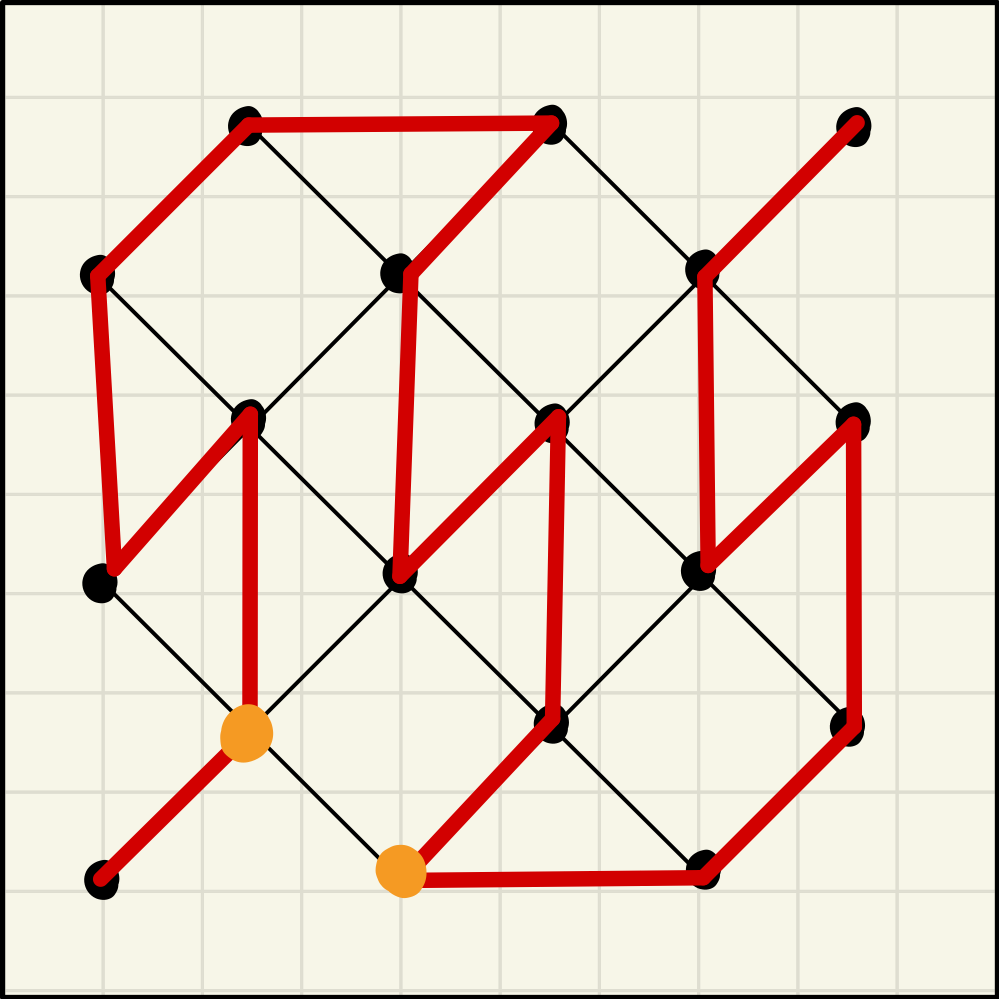
\includegraphics[width=0.4\textwidth]{figures/TFI/tenpy_snaking.jpeg}
\caption{An MPS can be put on a 2D square lattice by "snaking" it through the lattice. The two sites marked in orange are nearest neighbour sites in the lattice, but are far apart in the MPS. Thus, entanglement between the two sites is hard to represent, requiring large bond dimensions.}
\label{fig:tenpy_snaking}
\end{figure}
